\documentclass[10pt,a4paper]{article}
\usepackage[utf8]{inputenc}
\usepackage[italian]{babel}
\usepackage{amsmath}
\usepackage{amsfonts}
\usepackage{amssymb}
\usepackage[left=1cm,right=1cm,top=1cm,bottom=2cm]{geometry}
\usepackage{txfonts}
\usepackage[T1]{fontenc}
\usepackage[utf8]{inputenc}
\usepackage{graphicx}
\usepackage{wrapfig}
\usepackage{subcaption}
\usepackage{caption}
\usepackage{subcaption}
\usepackage{titlesec}
\setcounter{secnumdepth}{4}
\titleformat{\paragraph}
{\normalfont\normalsize\bfseries}{\theparagraph}{1em}{}
\titlespacing*{\paragraph}
{0pt}{3.25ex plus 1ex minus .2ex}{1.5ex plus .2ex}


\usepackage[none]{hyphenat}


\begin{document}
\subsection{Dal machine learning al deep learning}
Oggi l'intelligenza artificiale è un fiorente campo di ricerca, con l'obiettivo di risolvere una grande varietà di problemi, che per essere risolti attraverso la programmazione classica necessitano di una grande quantità di conoscenze pregresse, spesso non disponibili.\\
I Programmi basati sul paradigma dell'intelligenza artificiale si propongono di superare questi ostacoli acquisendo direttamente queste conoscenze dai dati grezzi, tale capacità è nota come machine learning.
Sotto questa famiglia di algoritmi si trovano altri sottogruppi quali il representation learning e all'interno di quest'ultimo il deep learning.\\ 
Il deep learning rispetto ai metodi più classici, tipicamente in grado di riconoscere relazioni lineari(come ad esempio il noto SVM o support vector machine), si propone come alternativa per l'apprendimento di funzioni a molte variabili non lineari anche molto complesse.
Le applicazioni più comuni comprendono il riconoscimento di oggetti nelle immagini, delle parole in tracce audio o anche per le traduzioni multilingue. \\
Il termine "deep learning" deriva proprio dalla capacità di questi modelli di riuscire a cogliere delle relazioni molto "profonde" tra i dati di ingresso e di uscita, approssimando con un certo errore ,dipendente dal caso specifico, la funzione che dati gli input restituisce l'output desiderato, purtroppo però presentano il grande problema di non rendere disponibile in maniera chiara le relazioni apprese.
   

\begin{figure}[h!]
  \centering
  \begin{subfigure}[t]{0.45\linewidth}
  	\centering
    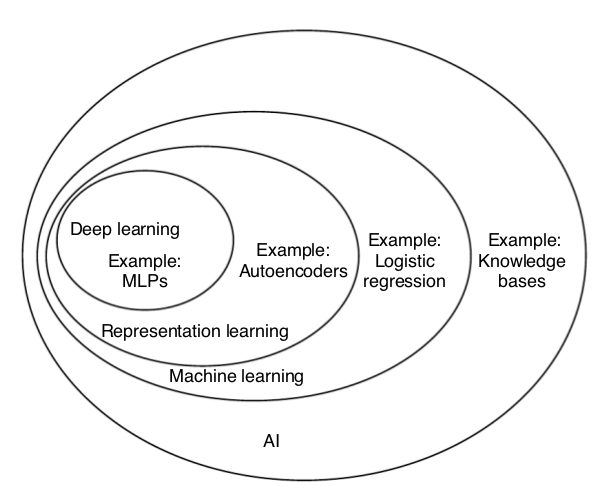
\includegraphics[height=200pt]{AI_venn_diagram.png}
    \caption*{famiglie di algoritmi}
  \end{subfigure}
  \begin{subfigure}[t]{0.45\linewidth}
  	\centering
    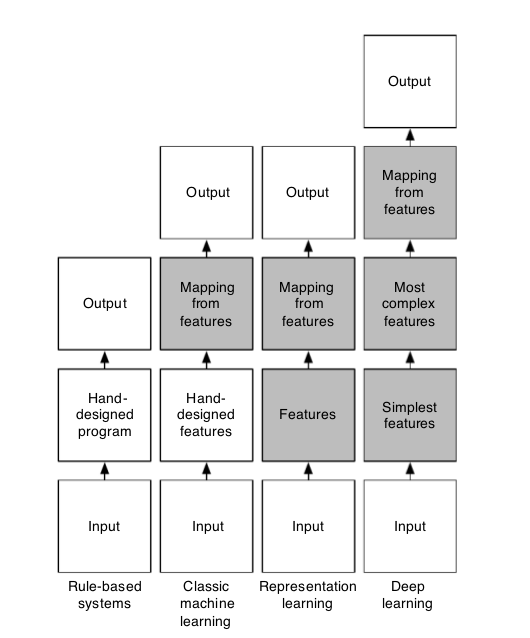
\includegraphics[height=200pt]{diff_between_aprochs.png}
    \caption*{differenze generali tra \\ le diverse tipologie di algoritmi}
  \end{subfigure}
  \label{fig:graph1}
\end{figure}

\subsubsection{Le reti feed-forward (MLP)}

\begin{wrapfigure}{r}{0.4\textwidth}
	\centering
	\vspace{-25pt}
    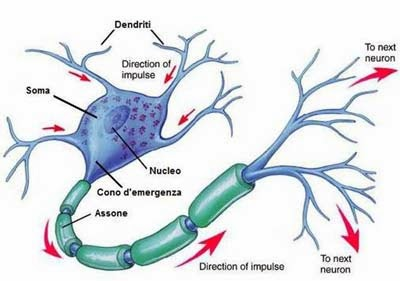
\includegraphics[width=0.4\textwidth]{neurone.jpg}
  	\caption{Il neurone biologico}
  	\label{fig:graph2}
  	\vspace{-20pt}
\end{wrapfigure}

Uno dei modelli della famiglia del deep learning più comuni e semplici da utilizzare sono le reti neurali feed-forward o multi layer perceptron, le quali sono assimilabili a modelli di regressione statistica.\\
Le reti neurali sono un modello matematico molto semplificato del\\ cervello, e per parlarne è necessario qualche riferimento al modello \\biologico.

\subsubsection*{Il neurone biologico}
L'unità base del cervello è rappresentata dai neuroni (Figuara \ref{fig:graph2}),\\ i quali a loro volta sono composti dai dendriti, dal soma, dall'assone e dalle sinapsi. 
\\I dendriti sono l'apparato di input del neurone, attraverso il quale riceve i segnali dall'ambiente o da altri neuroni, tali segnali caricano il neurone, che accumula un potenziale elettrico all'interno del soma.
In determinate condizioni o al raggiungimento di una certa soglia di potenziale il neurone emette un impulso lungo l'assone giungendo alle sinapsi, poste alla fine dell'assone, le quali sono connesse con altri neuroni o con altri apparati del corpo, come i muscoli.\\
Questa particolare cellula oltre a scambiare impulsi è in grado di accumulare informazioni attraverso l'ispessimento o l'assottigliamento della guaina mielinica, la quale è presente lungo l'assone.
Le variazioni dello spessore della guaina comportano un aumento o una diminuzione della resistenza elettrica dell'assone determinando una variazione dell'impulso percepito dai neuroni connessi alle sinapsi a parità di potenziale rilasciato.   

\newpage

\subsubsection*{Il percettrone} 

\begin{wrapfigure}{r}{0.4\textwidth}
	\centering
	\vspace{-15pt}
    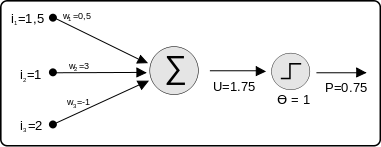
\includegraphics[width=0.4\textwidth]{percettrone.png}
  	\caption{Il percettrone}
  	\label{fig:graph3}
\end{wrapfigure}

Il neurone artificiale è composto da una serie di connessioni in ingresso, come i dendriti nel caso del neurone biologico, questa volta però il compito di immagazzinare informazione viene svolto da queste connessioni in input e non più dalle connessioni in output. 
Ad ogni input del neurone è associato un coefficiente che moltiplica il potenziale in ingresso, a questo punto gli ingressi pesati giungono al nodo sommatore, il corrispettivo del soma, che ne accumula la sommatoria.
Lo step successivo è il blocco contenente la funzione di trasferimento, una funzione che prende in input il potenziale del neurone e rende disponibile il risultato come output finale o come input per i neuroni successivi.
La funzione di trasferimento del neurone può essere di vari tipi, può variare infatti anche tra i neuroni della medesima rete, alcune delle più comuni \\sono:
\begin{wrapfigure}{r}{0.4\textwidth}
	\centering
	\vspace{-120pt}
    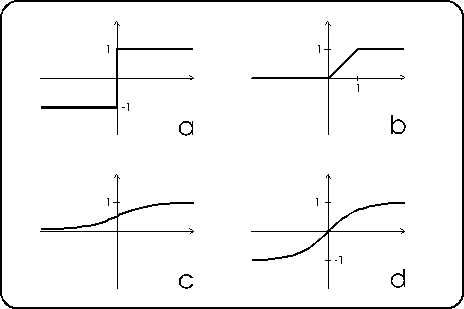
\includegraphics[width=0.4\textwidth]{FDTs.png}
  	\caption{Le funzioni di trasferimento}
  	\label{fig:graph4}
\end{wrapfigure}
(a) la funzione gradino. \\
(b) la funzione lineare con saturazione \\
(c) la funzione sigmoide tra 0 e 1 \\
(d) la funzione sigmoide tra -1 e 1 \\ \\
Volendo esprimere il percettrone in termini matematici si ottiene la seguente \\ equazione:

$\hspace*{100pt} y = f(P) = f(\textstyle\sum_i W_i \cdot X_i)$\\
\(\mathnormal{y}\) - output del percettrone\\
\(\mathnormal{f}\) - funzione di trasferimento del percettrone\\
P - potenziale del neurone\\
\(W_i\) - peso o coefficiente dell'i-esimo ingresso\\
\(X_i\) - potenziale d'ingresso dell'i-esimo neurone\\
\\Una delle caratteristiche più importanti del percettrone è la sua capacità di compiere separazioni lineari. Tali separazioni avvengono in uno spazio a n dimensioni, dove n corrisponde al numero di variabili in ingresso al neurone, perciò si avrà ad esempio per un percettrone a due input la capacita di separare i valori su \(\Re^2\) attraverso un retta, nel caso \(\Re^3\) si potranno separare i valori dello spazio tridimensionale attraverso un piano, e così via.\\
\begin{figure}[h!]
  \centering
  \begin{subfigure}[t]{0.45\linewidth}
  	\centering
  	%\hspace{-120pt}
    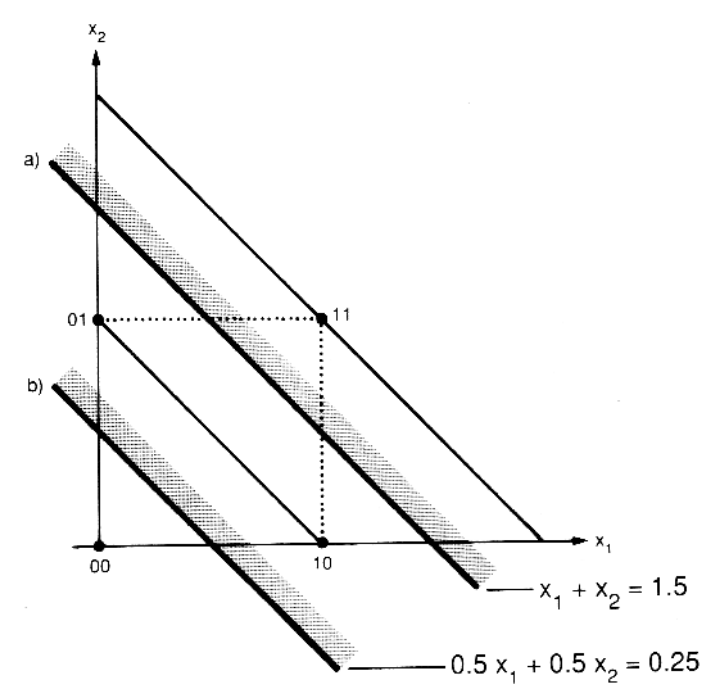
\includegraphics[height=240pt]{sepAndOr.png}
    \captionsetup{justification=centering}
    \caption*{esempio di linee di separazione per neurone a 2 ingressi binari\\
    (a - funzione OR)\\
    (b - funzione AND)}
  \end{subfigure}
  \begin{subfigure}[t]{0.45\linewidth}
    %\hspace{-200pt}
  	\centering
    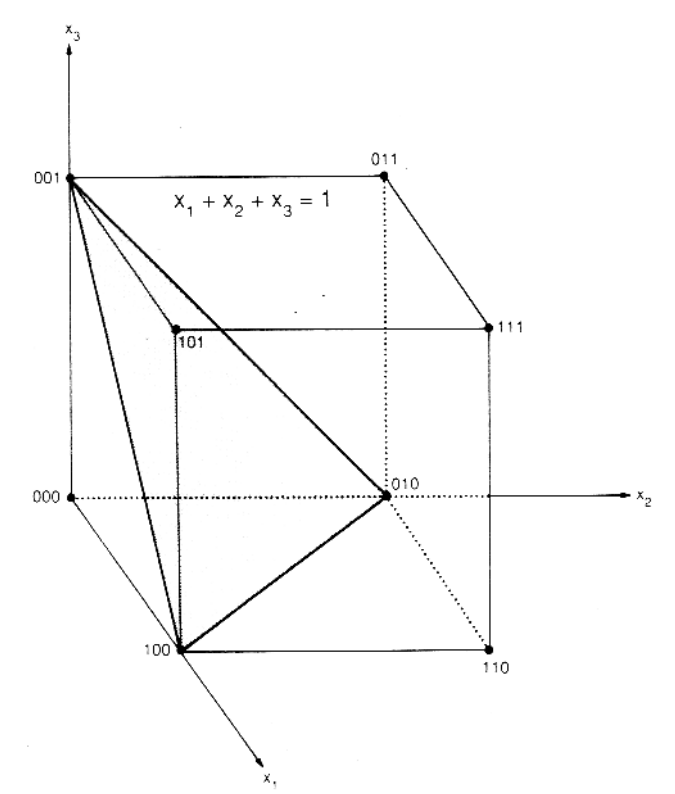
\includegraphics[height=240pt]{sepR3.png}
    \captionsetup{justification=centering}
    \caption*{esempio di piano diseparazione lineare \\ a 3 ingressi per un neurone binario}
  \end{subfigure}
  \label{fig:graph5}
\end{figure}
\\ \\

\subsubsection*{Le reti multi-strato e la separazione non lineare} 
Le reti multi-strato sono composte da strati di percettroni, interconnessi tra loro in modo che gli output degli strati precedenti siano connessi con gli input dei percettroni successivi. Tale struttura "profonda" permette di rappresentare funzioni non linerai molto complesse, tanto più sono gli strati della rete.\\
Uno degli esempi che meglio chiarisce questa problematica è la funzione xor nel seguente esempio, la quale per semplicità è rappresentata con neuroni binari a soglia.

\subsubsection*{Il problema dello XOR}
Lo xor è una delle funzioni non lineari più semplice, nella quale diventa evidente l'impossibilità di approssimare tale funzione con un solo strato di neuroni.
Il grafico illustra come un neurone singolo possa effettuare la separazione lineare che riproduce la funzione and e or, ma come si nota lo xor necessità di due parabole per la separazione e non più di rette, tale separazione si effettua utilizzando una rete ad almeno due strati. 
%
\begin{figure}[h!]
  \centering
  \begin{subfigure}[t]{0.45\linewidth}
  	\centering
  	%\hspace{-120pt}
    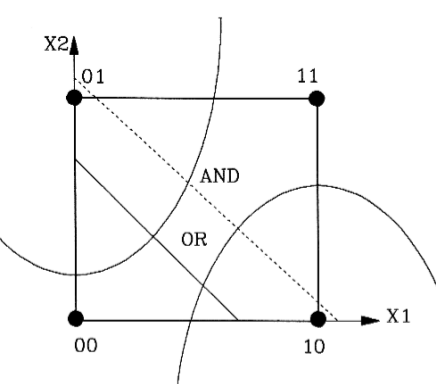
\includegraphics[height=140pt]{SepXor.png}
    \captionsetup{justification=centering}
    \vspace{10pt}
    \caption*{Esempio di linee di separazione per and or e xor}
  \end{subfigure}
  \begin{subfigure}[t]{0.45\linewidth}
    %\hspace{-200pt}
    \vspace{-130pt}
  	\centering
    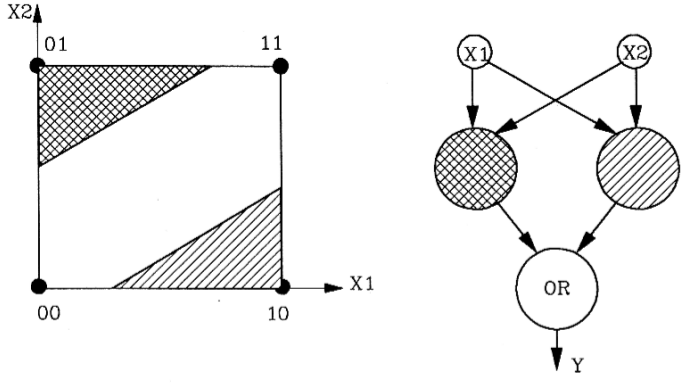
\includegraphics[height=140pt]{MLPxor.png}
    \captionsetup{justification=centering}
    \caption*{MLP in grado di rappresentare la funzione xor}
  \end{subfigure}
  \label{fig:graph6}
\end{figure}
%
\subsubsection{La funzione di addestramento: Il back-propagation} 
Come già detto la struttura della rete neurale deve apprendere una data funzione da dei dati.\\
Tale operazione si effettua presentando degli input alla rete ai quali questa risponderà con degli output, i quali dovranno essere confrontati con degli output corretti per il set di input presentato, per calcolare l'errore nell'output della rete.\\
L'errore che la rete commette ad ogni tentativo viene utilizzato per calcolare attraverso una prescelta funzione, nel nostro caso il BP, dei coefficienti di correzione che vanno applicati ai pesi della rete per avvicinare il suo output a quello desiderato. \\
Come dice il nome "retropropagazione" in italiano, l'errore calcolato dall'output viene applicato ai neuroni precedenti e poi a quelli ancora precedenti fino ad arrivare al primo strato, tale procedura puo essere effettuata in diversi modi, calcolando gli errori su un determinato numero di esempi del dataset, accumulando le correzioni ed applicandole successivamente, tale tecnica è attualmente la più utilizzata ed è detta "mini-batch", ma è possibile anche effettuare la correzione esempio per esempio, e questo è detto addestramento in-line, in fine tra i metodi più comuni c'è anche la possibilità di eseguire tutti gli esempi del dataset e solo alla fine di un'intero ciclo di addestramento applicare le correzioni. questi tre metodi ovviamente risultano validi ma a seconda del problema da risolvere possono avere prestazioni migliori o peggiori in modo difficilmente prevedibile.
\\
Dopo questa introduzione generale all'addestramento delle reti passiamo a dare una vista più accurata dell'algoritmo utilizzato nel progetto che è principalmente pensato per reti mlp con neuroni ad ingressi continui e con funzione di trasferimento sigmoidea o ad arcotangente.
\\
Il BP cerca di minimizzare l'errore quadratico medio, relativo a un training set di esempi dati, scendendo lungo la superficie d'errore e seguendo la direzione di massima pendenza, in cerca di una "valle" sufficientemente profonda. \\
Consideriamo una rete con n input $X_i$ (i = 1, 2,.. n), uno strato nascosto di q neuroni $Z_k$ (k = 1, 2..., q) e uno strato output di m neuroni $Y_j$; (j = 1, 2... m).
Il training set sia costituito da p esempi o casi $C_r$, (r = 1, 2,..,p). Tutti i neuroni abbiano la stessa funzione di trasferimento.\\
L'errore quadratico medio dello strato output è:\\ \\
\begin{equation} \label{eq:eqm}
E = \frac{1}{2} \sum_j{\sum_r{(Y_{rj} - D_{rj})^2}}
\end{equation}

dove Y, è l'output del neurone $Y_j$ alla presentazione dell'esempio $C_r$ e $D_{rj}$ è il
suo valore desiderato. Per semplificare la notazione, eliminiamo l'indice r e minimizziamo l'errore quadratico medio ad ogni presentazione di esempio (modalità on-line), anziché dopo ogni ciclo completo di presentazione del training set
o epoca (modalità batch). Avremo allora:
\\ \\
\begin{equation} \label{eq:eq}
E = \frac{1}{2} \sum_j{(Y_{j} - D_{j})^2}
\end{equation}
\\ \\
Si applica a questo punto la regola del gradiente (fig. Propagazione a):

\begin{equation} \label{eq:grad}
\Delta W_{jk} = - \eta \frac{\partial E}{\partial W_{jk}} = - \eta \frac{\partial E}{\partial Y_j} \frac{\partial Y_j}{\partial P_j} \frac{\partial P_j}{\partial W_{jk}} = 
-\eta(Y_j - D_j)f'(P_j)Z_k
\end{equation} \\
\begin{equation} \label{eq:dey}
\frac{\partial E}{\partial Y_j} = (Y_j - D_j)
\end{equation} \\
\begin{equation} \label{eq:dyp}
\frac{\partial Y_j}{\partial P_j} = f'(P_j) 
\end{equation} \\
\begin{equation} \label{eq:dpw}
\frac{\partial P_j}{\partial W_{jk}} = \frac{\partial(\sum W_{jk} Z_k)}{\partial W_{jk}} = Z_k
\end{equation}

Ponendo a questo punto:
\begin{equation} \label{eq:cr}
\delta_j = (Y_j - D_j)f'(P_j) 
\end{equation}
\\
\begin{equation} \label{eq:gradcr}
\Delta W_{jk} = -\eta \ \delta_j \ Z_k
\end{equation}
La formula (\ref{eq:grad}) viene impiegata per aggiornare i pesi sinattici delle connessioni tra strato nascosto e strato output, analogamente, per quanto riguarda le connessioni tra strato input e strato nascosto si utilizza la formula (fig. Propagazione b):
\begin{equation} \label{eq:dih}
\Delta W_{ki} = -\eta \frac{\partial E}{\partial W_{ki}} = - \eta \frac{\partial E}{\partial Z_k} \frac{\partial Z_k}{\partial P_k} \frac{\partial P_k}{\partial W_{ki}} = -\eta \frac{\partial E}{\partial Z_k}f'(P_k)X_i
\end{equation}
Confrontando questa formula con la precedente formula (\ref{eq:grad}), al posto degli errori noti $(Y_j - D_j)$ troviamo le derivate $\frac{\partial E}{\partial Z_k}$, che dobbiamo ora calcolare retropropagando l'errore dallo strato output a ogni neurone nascosto:
\begin{equation} 
\frac{\partial E}{\partial Z_k} = \sum_j \Bigg( \frac{\partial E}{\partial Y_j} \frac{\partial Y_j}{\partial P_j} \frac{\partial P_j}{\partial Z_k} \Bigg) = \sum_j (Y_j - D_j)f'(P_j)W_{jk} 
\end{equation}

o anche, applicando la formula (\ref{eq:cr}) :
\begin{equation}
\frac{\partial E}{\partial Z_k} = \sum_j \ \delta_j \ W_{jk}
\end{equation}
\begin{figure}[h!]
  	\centering
  	%\hspace{-105pt}
    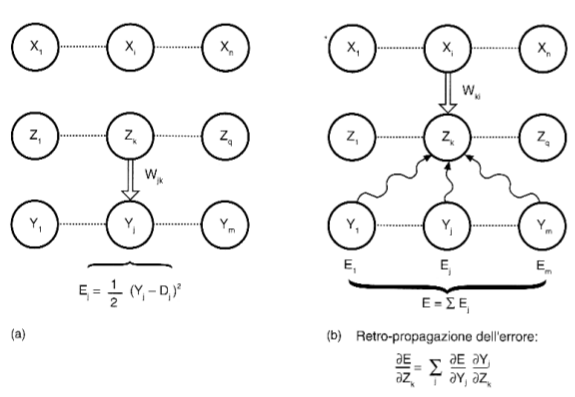
\includegraphics[height=300pt]{PropagationGraph.png}
    \captionsetup{justification=centering}
    \caption*{Propagazione dell'errore nella rete}
  \label{fig:graph7}
\end{figure}
\\
In fine otteniamo le equazioni:
\begin{equation} \label{eq:dih}
\Delta W_{ki} = -\eta f'(P_k)(\sum_j \delta_j W_{jk})X_i
\end{equation}
che ponendo:
\begin{equation} \label{eq:dbpk}
\delta_k = f'(P_k)(\sum_j \delta_j W_{jk})
\end{equation}
la quale assume la stessa forma della (\ref{eq:gradcr}) :
\begin{equation} \label{eq:dpk}
\Delta W_{ki} = -\eta \ \delta_k \ X_i
\end{equation}
Le formule (\ref{eq:dih}) (\ref{eq:dbpk}) (\ref{eq:dpk}) sono valide non solo per aggiornare i pesi sinattici tra strato nascosto (l’unico nella rete che abbiamo ipotizzato) e strato input ma anche, in reti più generali, per le connessioni tra due strati nascosti consecutivi.
Se si adotta la funzione di trasferimento sigmoide si ha:

\begin{equation}
Y = f(P) = \frac{1}{1+e^{kP}}
\end{equation}
\begin{equation}
f'(P) = kf(P)(1-f(P)) = kY(1-Y)
\end{equation}
Dove k è proporzionale alla pendenza della sigmoide nel suo punto di flessione, normalmente si pone k = 1.
A questo punto otteniamo la rielaborazione delle formule (\ref{eq:gradcr}) (\ref{eq:dih}):
\begin{equation}
\Delta W_{jk} = -\eta k (Y_J - D_j)Y_j(1-Y_j)Z_k
\end{equation} 
\begin{equation}
\Delta W_{ki} = -\eta k Z_k (1-Z_k)(\sum_j \delta_j W_{jk})X_i
\end{equation} 
infine i pesi sinattici vengono aggiornati, ad ogni tempo t dell'intervallo 1, 2, ..., (t-1), t, (t+1), ...ecc con:
\begin{equation}
W_{jk}(t+1) = W_{jk}(t) + \Delta W_{jk}
\end{equation}
\begin{equation}
W_{ki}(t+1) = W_{ki}(t) + \Delta W_{ki}
\end{equation} 
\end{document}